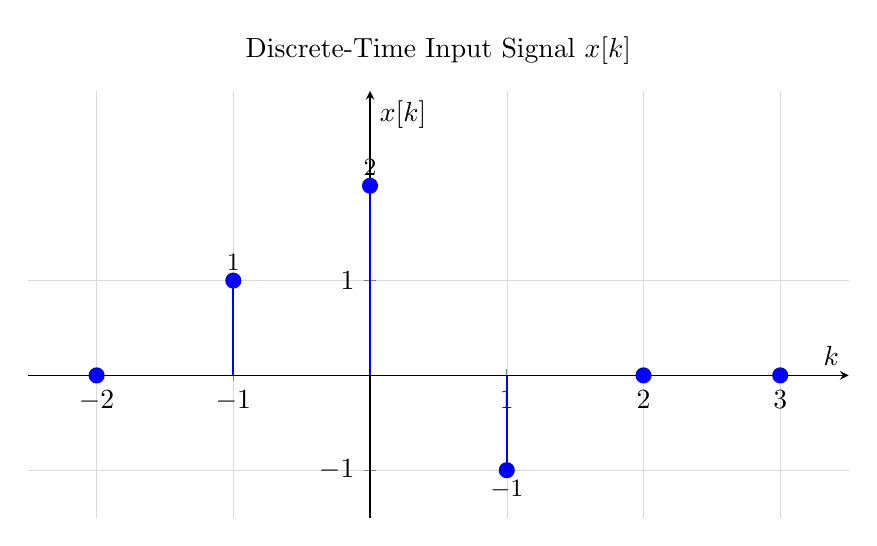
\begin{tikzpicture}
	% Define a style for our stem plots
	\pgfplotsset{
		impulse/.style={
			ycomb,
			blue,
			thick,
			mark=*,
			mark size=2.5pt,
			mark options={fill=blue, draw=blue},
		}
	}
	
	\begin{axis}[
		width=12cm,
		height=7cm,
		title={Discrete-Time Input Signal $x[k]$},
		xlabel={$k$},
		ylabel={$x[k]$},
		axis lines=middle,
		xmin=-2.5, xmax=3.5,
		ymin=-1.5, ymax=3,
		xtick={-2, -1, 0, 1, 2, 3},
		ytick={-1, 1},
		grid=major,
		grid style={line width=.1pt, draw=gray!30},
		]
		
		% Plot positive values with labels above
		\addplot[
		impulse,
		nodes near coords,
		every node near coord/.style={anchor=south, font=\small, text=black},
		] coordinates {(-1,1) (0,2)};
		
		% Plot negative values with labels below
		\addplot[
		impulse,
		nodes near coords,
		every node near coord/.style={anchor=north, font=\small, text=black},
		] coordinates {(1,-1)};
		
		% Plot zero-value points
		\addplot[impulse] coordinates {(-2,0) (2,0) (3,0)};
		
	\end{axis}
\end{tikzpicture}